\chapter{Design and Structure}
\label{Chapter4} 
Through results gathered from the previous chapter according analyzing and specifying the requirements of the project, we can now start the design step as it is a crucial and aim to undertake and prepare the ground for the implementation step. In this chapter, we will present our conceptual approach as well as arguments for this choice. Then we explain the detailed design.
\section{Global Design}


\subsection{Architectural Overview}
 
Figure \ref{phy} shows the physical architecture of the system. It includes the different material component that build our applications infrastructure.  
 ~\\
\begin{figure}[!ht]
\begin{center}
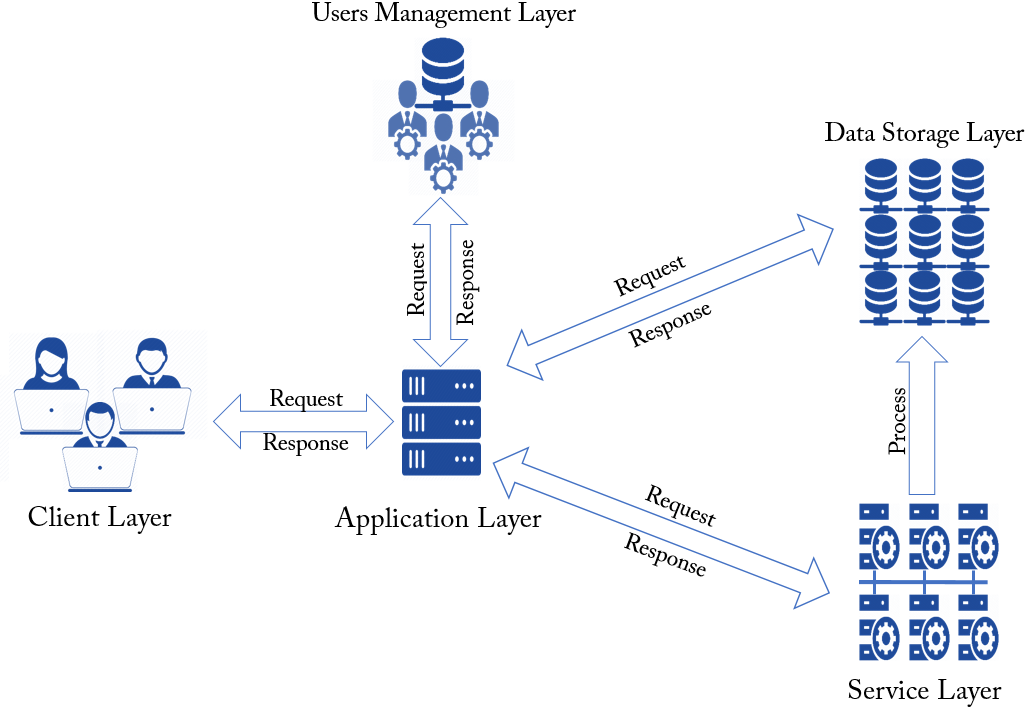
\includegraphics[width=17cm,height=10.2cm]{chapter4/fig1.png}
\end{center}
\caption{General Architecture of the System}
\label{phy}
\end{figure}
 
The software physical architecture is structured around 5 main layers. Every layer presents a different physical level of the application structure.
\begin{itemize}
\item \textbf{Client Layer:} is a display level of the application, includes the web view in the users browser.\\ 
\item \textbf{Application Layer:} is the web server, the module that executes the different component of our application core.\\
\item \textbf{Users Management Layer:} is data base server that contains the application users information, which make it possible for the application layer to manage users and their roles.\\
\item \textbf{Service Layer:} is the layer where the Spark core executes. It composed from a master cluster and many worker nodes dispersed in different clusters.\\
\item \textbf{Data Storage Layer:} is the layer where files are managed through Hadoop Distributed File System. This layer is composed from many clusters, each cluster is composed from many servers.\\
\end{itemize}
\subsection{Software Architecture}

Figure \ref{package} shows the software internal architecture. This architecture is illustrated through a package diagram.\\

\begin{figure}[!ht]
\begin{center}
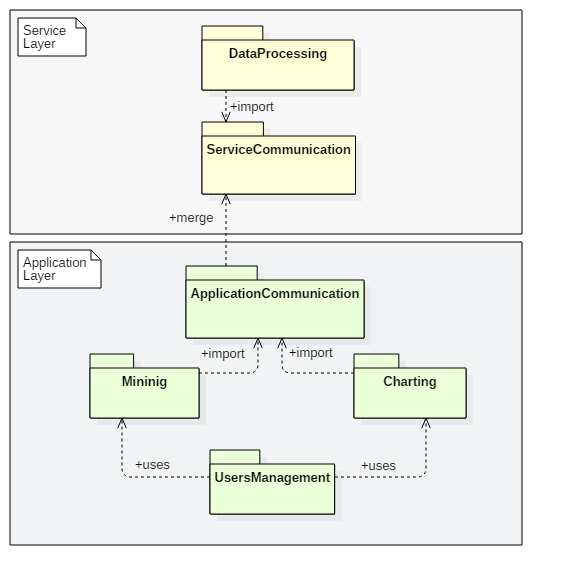
\includegraphics[width=15cm,height=10cm]{chapter4/package.png}
\end{center}
\caption{Packages Diagram}
\label{package}
\end{figure}

\begin{itemize}
\item \textbf{Service Layer:}\\
\begin{itemize}
\item \textbf{DataProcessing:} Contains Python classes that are supposed to execute Spark core. This package is a processing \\
\item \textbf{ServiceCommunication:} In this package we find all component needed to maintain communication between the service layer and the application layer through sockets queries.\\
\end{itemize}

\item \textbf{Application Layer:}\\
\begin{itemize}
\item \textbf{ApplicationCommunication:} is the application layer image for the ServerCommunication package. It communicates with the service layer through sockets queries.\\
\item \textbf{Mining:} is the package that gathers the different models of the used algorithms. This algorithm does not really execute the algorithm but it set the algorithm parameters in order to send it through sockets queries to the service layer that will be responsible to execute the desired algorithm.\\
\item \textbf{Charting:} For every algorithm model, there is a charting model which will present a personalized way the execution algorithm results.\\
\item \textbf{UserManagement:} is the layer that covers all model of user management such login, logout and roles given for each type of users.\\
\end{itemize}
\end{itemize}




\section{Detailed Design}
\subsection{Class Diagram}
Figure \ref{class} shows the class diagram of our proposed solution. Every class is presented on its containing package.\\

\begin{itemize}
\item \textbf{Service Layer:}\\
\begin{itemize}
\item \textbf{Kmeans:} Kmeans class is the controller class that executes the kmeans algorithm in Saprk core. its parameters are set through the received data from the application layer.\\
\item \textbf{Pca:} PCA class is the controller class that executes the PCA algorithm in Saprk core. its parameters are set through the received data from the application layer.\\
\item \textbf{DecisionTree:} DecisionTree class is the controller class that executes the decision Tree algorithm in Saprk core. its parameters are set through the received data from the application layer.\\
\item \textbf{LinearRegression:} LinearRegression class is the controller class that executes the Linear Regression algorithm in Saprk core. its parameters are set through the received data from the application layer.\\
\item \textbf{SocketServer:} SocketServer is class in service layer that implements all needed methods to make the executing service in permanent communication with the application.\\
\end{itemize}

\item \textbf{Application Layer:}\\
\begin{itemize}
\item \textbf{SocketClient:} SocketClient is the image class for the SocketServer in service side. It implements all the needed methods to communicate those from the socket server side (service layer).\\
\item \textbf{Pca:} Pca class is a model that make the application user sets the algorithms parameters and launch its execution in the service side.\\
\item \textbf{Kmeans:} Kmeans class is a model that make the application user sets the algorithms parameters and launch its execution in the service side.\\
\item \textbf{DecisionTree:} DecisionTree class is a model that make the application user sets the algorithms parameters and launch its execution in the service side.\\
\item \textbf{LinearRegression:} LinearRegression class is a model that make the application user sets the algorithms parameters and launch its execution in the service side.\\
\item \textbf{PcaChart:} PcaChart is the controller of the pca result chart load.\\
\item \textbf{KmeansChart:} KmeansChart is the controller of the pca result chart load.\\
\item \textbf{DecisionTreeChart:}  DecisionTreeChart is the controller of the pca result chart load.\\
\item \textbf{LinearRegressionChart:}  LinearRegressionChart is the controller of the pca result chart load.\\
\item \textbf{User:} User a class is a mother class that define all the common attributes and methods for any user type.\\
\item \textbf{Administrator:} Administrator class inherits all the methods and attributes from the User mother class. It define on type of users' roles by adding its own specific methods.\\
\item \textbf{Client:} Client is a specified class defined to represent a client type user. It inherits from the User mother class and implement its own specified methods.\\
\end{itemize}
\end{itemize} 


\begin{figure}[!ht]
\begin{center}
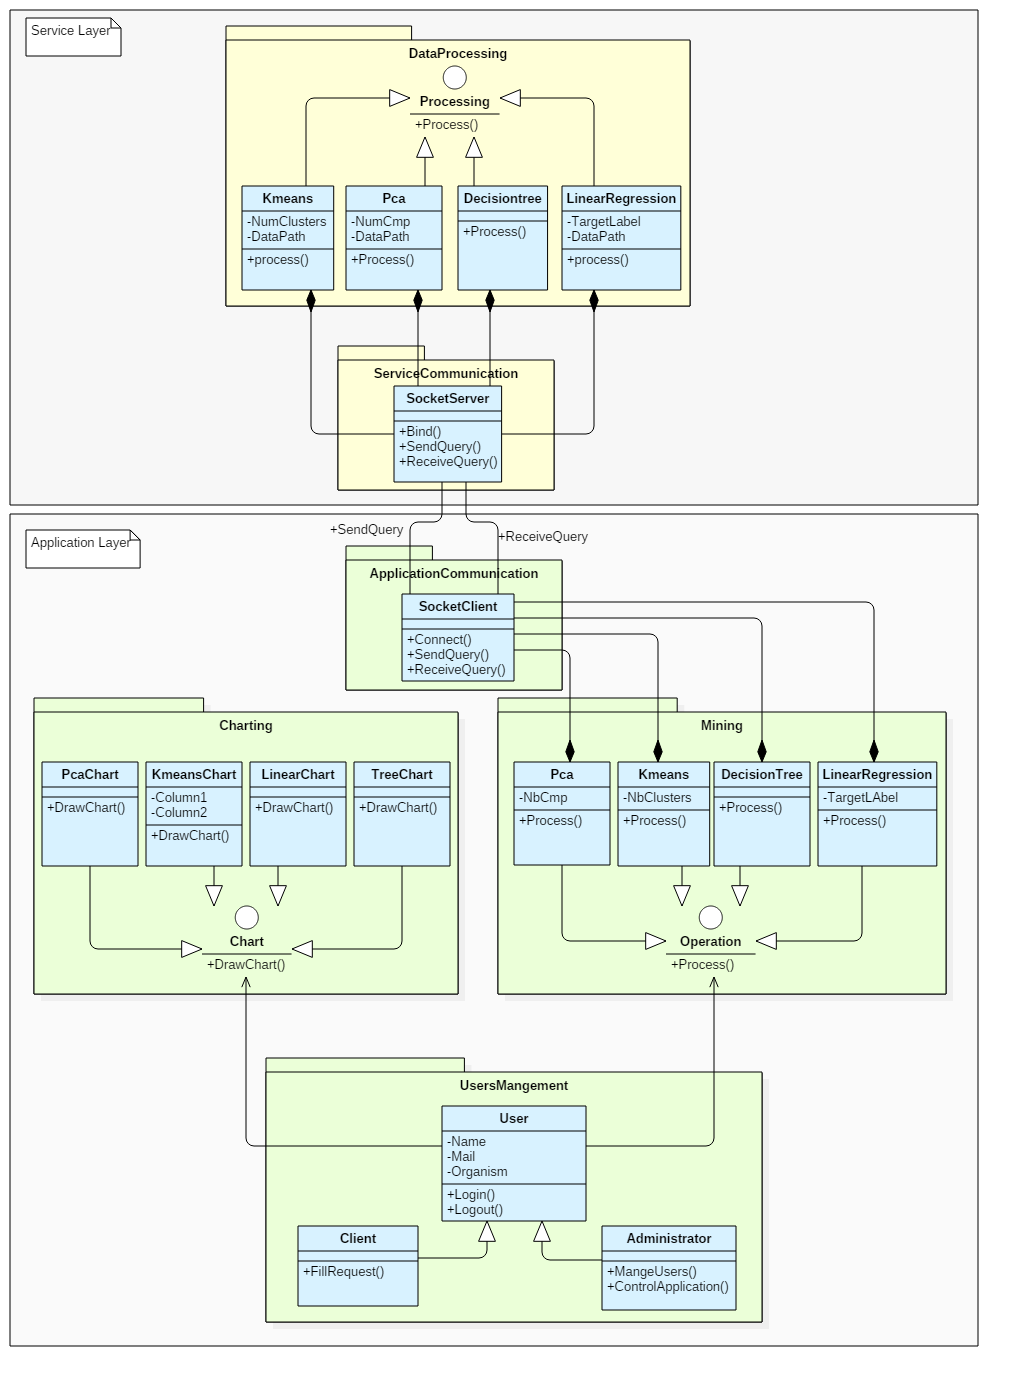
\includegraphics[width=17cm,height=23.5cm]{chapter4/class.png}
\end{center}
\caption{Class Diagram}
\label{class}
\end{figure}


\subsection{Sequences Diagrams}
\subsubsection{General Sequence Diagram}

Our system is mainly composed from 4 components; client side web application, a web server connected to a SQL data base to manage users accounts, a service server that runs operations on the data and many data storage servers. Figure \ref{seq0} shows the interaction between these different components when a user perform a single operation.\\

First the client types his login and password in the login form, the web server check in his data base and return either a failure notification ("wrong login and password") or a successful connection session to the client.\\

Throughout this session, the client can send a data load request to the web server, which will load data in data storage servers; if the operation is correctly done the user will be notified. In another step, the client will process an algorithm on a selected data. He will, then, select data and set the algorithm parameters. The web server will transfer this information to service server, which will run the algorithm and return a result file in a success case or an error notification otherwise. \\

The user can also load charts from the generated result files. He sets the chart parameter and the web server will take charge to draw the appropriate chart. \\

After finishing his job, the client can disconnect and the server will destroy the user session.\\

\newpage
\begin{figure}[!ht]
\begin{center}
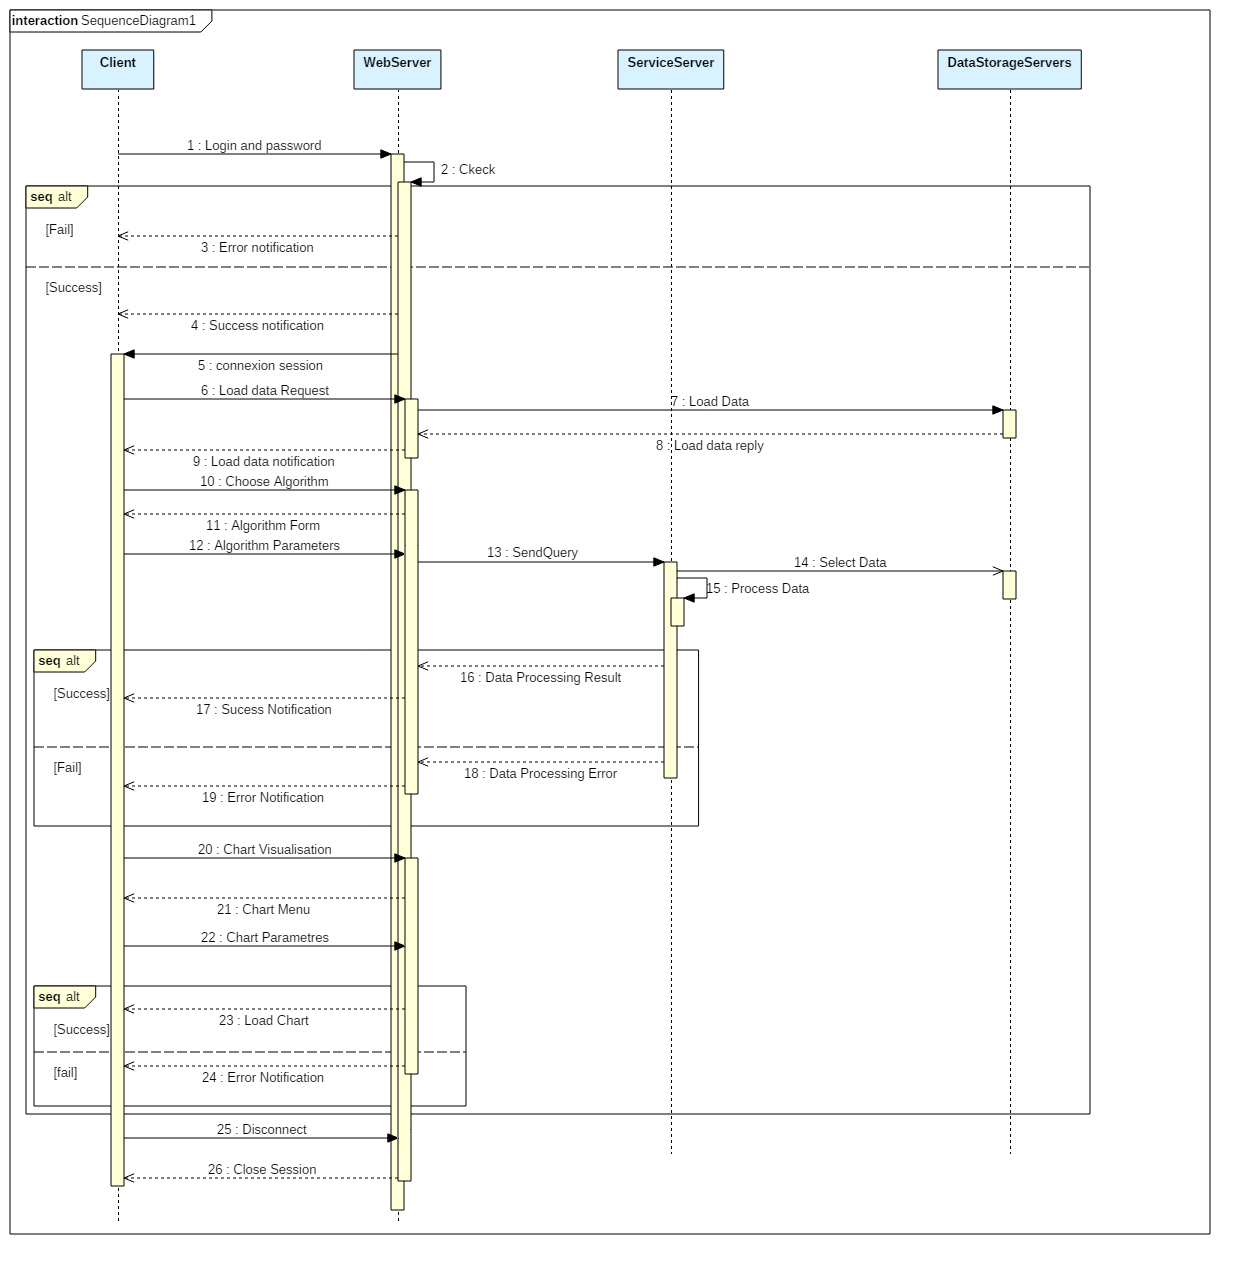
\includegraphics[width=17cm,height=24cm]{chapter4/sequence.png}
\end{center}
\caption{General Sequence Diagram}
\label{seq0}
\end{figure}
\subsubsection{Optimum Communication scenario}

Figure \ref{seq1} is a sequence diagram showing the optimum scenario of the connection established between the application server and the service server. This figure shows also the queries acknowledgement system that we have adopted to transfer the selected parameters from the user interface to the service server. First, the application ask for a TCP/IP connection. The service server establish the connection and create an appropriate thread for the actual operation. Then the application server send one parameter and wait for an acknowledgement  the send the next one. After sending all the needed parameters, the connection break down and the service server kill the operation thread. 

\begin{figure}[!ht]
\begin{center}
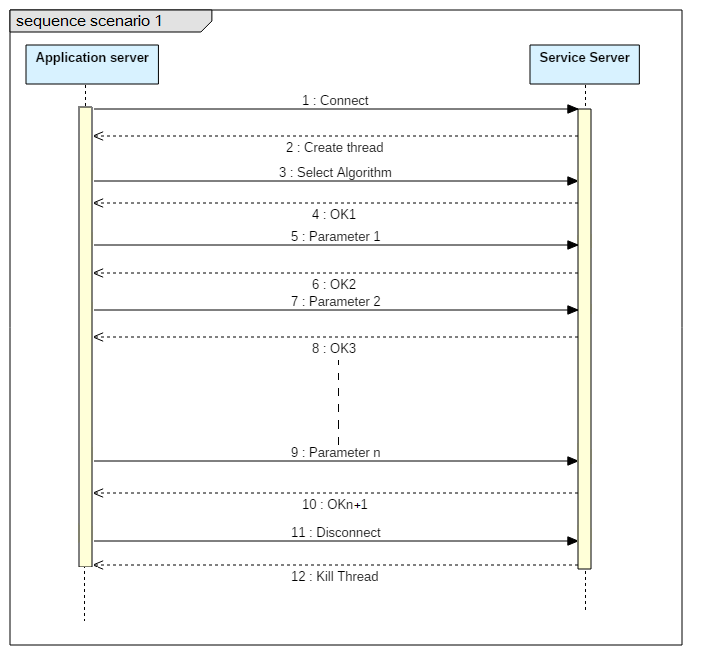
\includegraphics[width=12cm,height=13cm]{chapter4/SequenceDiagram1.png}
\end{center}
\caption{Optimum Communication scenario}
\label{seq1}
\end{figure}



\subsubsection{Lost Query Scenario}
Queries are the main way to make the application server and service server communicate. Queries are sent through TCP/IP sockets. In order to avoid server overload, if a query is lost the receiver will not wait for it infinitely. After exceeding a predefined timeout, the application layer will sent a query to disconnect from the service and then kill the attached service thread.\\

Figure \ref{seq2} describes this previously mentioned scenario.

\begin{figure}[!ht]
\begin{center}
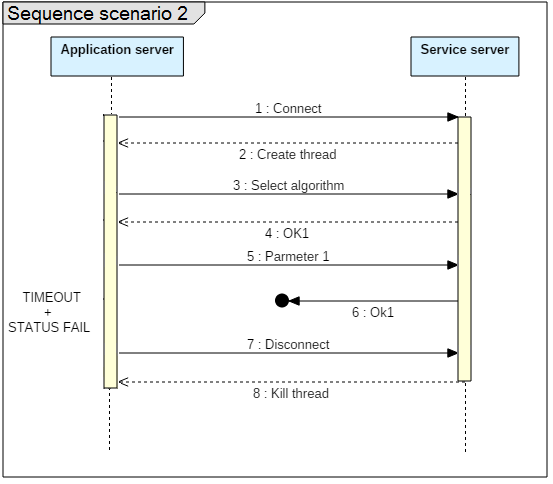
\includegraphics[width=9.3cm,height=8cm]{chapter4/SequenceDiagram2.png}
\end{center}
\caption{Lost Query Scenario}
\label{seq2}
\end{figure}




\subsubsection{Multi-Thread Communication Query Scenario}
In Order to grantee a multi-users application, we have adopted a multi-thread solution.  For every operation running in the service, we create a thread. As we are using a socket solution to send communication queries between the application server and the service server, there is a threat that a query sent from one thread disturb another one. In order to avoid the risk of disturbing the application, every sent or received query should be preceded by a user id in order to identify every query to whom user's thread belongs. If a thread receive a query that does not mind him, it will reject it and then inform the application server to send a query again. For every query received, the service thread make the same job, until it receive the correct query or reaches a maximum number of iterations; if it overcome it, it will reject the whole operation and kill the thread in order to avoid server overload and sudden shutdown.\\

Figure \ref{seq3} describes this previously mentioned scenario.  

\begin{figure}[!ht]
\begin{center}
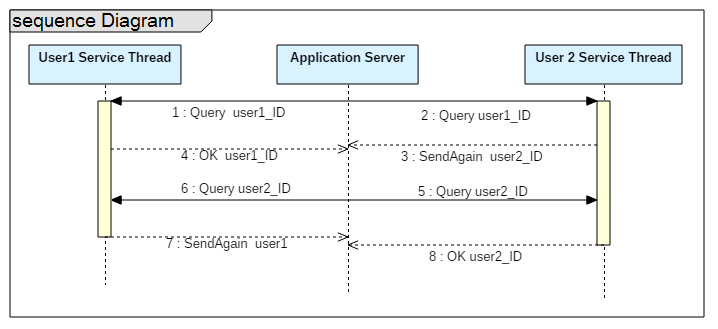
\includegraphics[width=11.5cm,height=7.5cm]{chapter4/SequenceDiagram3.png}
\end{center}
\caption{Multi-Thread Communication Query Scenario}
\label{seq3}
\end{figure}


\section*{Conclusion}

This chapter set the main guidelines on how we expect our solution to be. We started by giving an overview of our solution along with its physical architecture. Then, we provided various diagrams such as package, class and sequence diagrams to give more details on our solution's structure and interaction between its different elements. Since we agreed on the design of our solution, the next chapter will focus on the implementation
and the results we have reached.